\documentclass[a4paper,12pt]{article}
% --- Miglioramento grafica ---
\usepackage{titlesec} % Per personalizzare titoli
\usepackage{fancyhdr} % Per intestazioni e piè di pagina
\usepackage{xcolor}   % Per colori
\usepackage{tcolorbox} % Per riquadri e box
\usepackage{lmodern}  % Font più moderno
\usepackage{enumitem} % Migliore gestione elenchi
\usepackage[utf8]{inputenc}
\usepackage{amsmath, amssymb}
\usepackage{geometry}
\usepackage{graphicx}
\usepackage{hyperref}
\geometry{margin=2.5cm}

% Colori personalizzati
\definecolor{myblue}{RGB}{0, 102, 204}
\definecolor{mygray}{RGB}{240, 240, 240}

% Titoli sezioni colorati e moderni
\titleformat{\section}{\normalfont\Large\bfseries\color{myblue}}{\thesection}{1em}{}
\titleformat{\subsection}{\normalfont\large\bfseries\color{myblue}}{\thesubsection}{1em}{}

% Intestazione e piè di pagina
\pagestyle{fancy}
\setlength{\headheight}{14.5pt}
\fancyhf{}
\fancyhead[L]{\color{myblue}Relazione Database}
\fancyhead[R]{\color{myblue}Gino Pandozzi-Trani}
\fancyfoot[C]{\thepage}

% Elenchi con pallini blu
\setlist[itemize]{label=\textcolor{myblue}{\textbullet}}


\begin{document}

% --- Frontespizio migliorato ---
\begin{tcolorbox}[colback=mygray,colframe=myblue,width=\textwidth,arc=6mm,boxrule=1.2pt]
    \begin{center}
        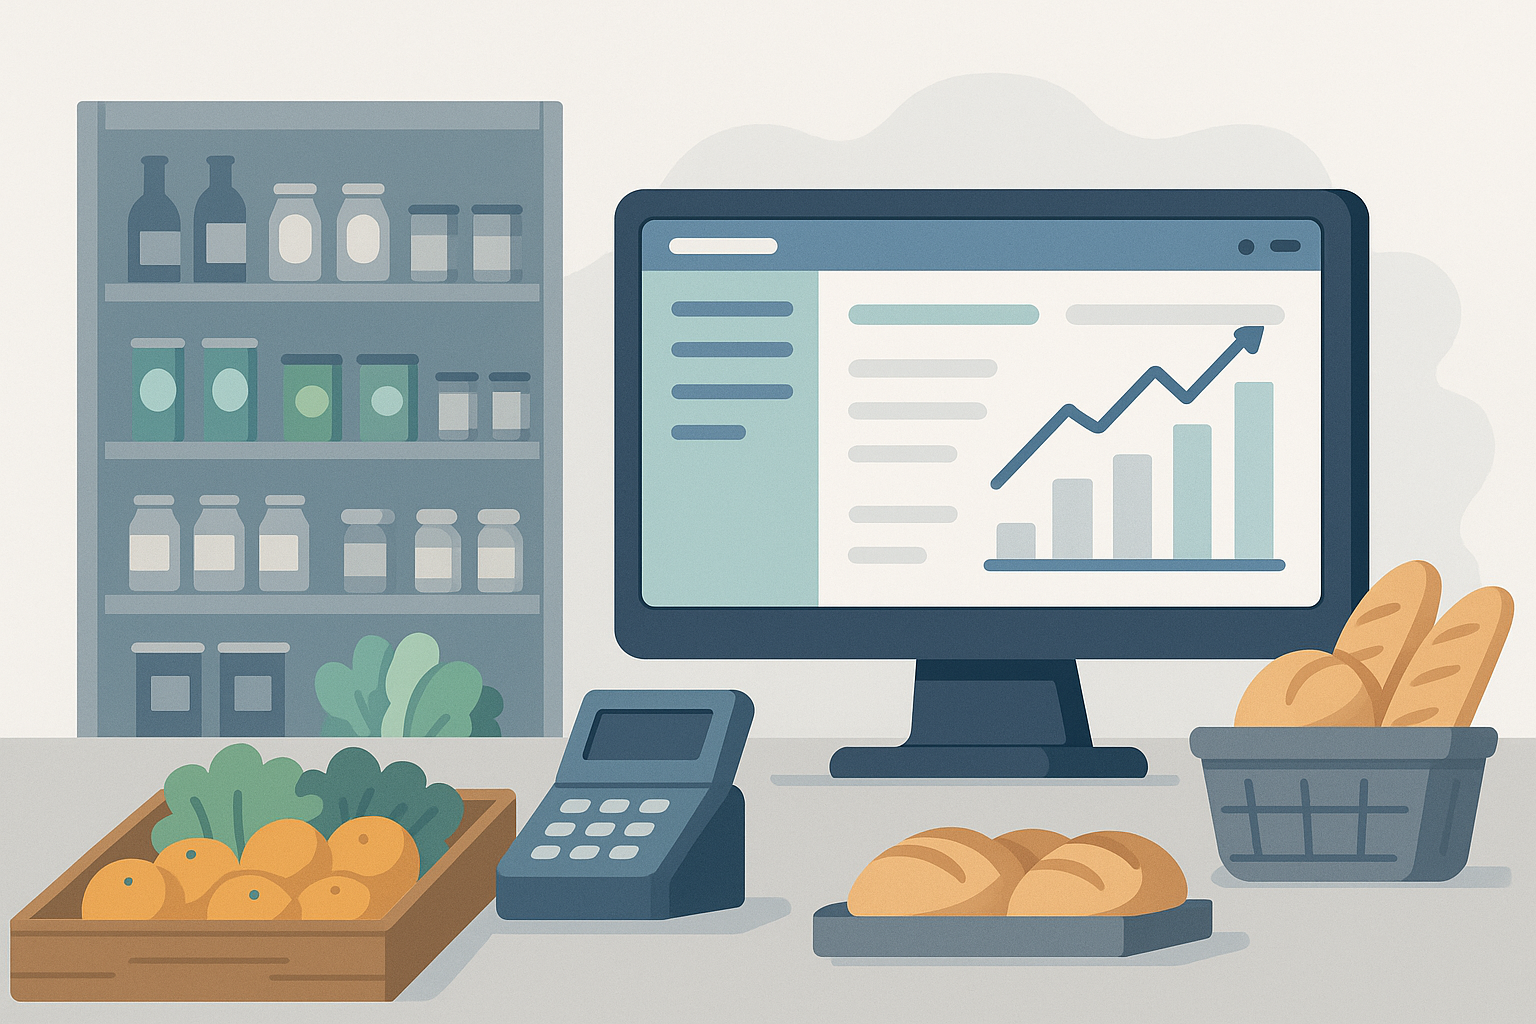
\includegraphics[width=0.6\textwidth]{../Immagini/Frontespazio.png} \\
        \vspace{1cm}
        {\Huge\bfseries\color{myblue} Sistema di Gestione per un Negozio di Alimentari} \\
        \vspace{1cm}
        {\Large\color{black} Autore: Gino Pandozzi-Trani} \\
        \vspace{0.5cm}
        {\large\color{black} Luglio 2025}
    \end{center}
\end{tcolorbox}


\newpage
\tableofcontents

\newpage
\section{Introduzione}
SISTEMA DI GESTIONE PER UN NEGOZIO DI ALIMENTARI
Si sviluppi un sistema informativo, composto da una base di dati relazionale e un applicativo Java dotato di
GUI (Swing o JavaFX), per la gestione di un sistema di un negozio di ortofrutta. Il sistema deve permettere di
gestire le vendite e la disponibilità dei prodotti disponibili, identificando le tipologie (frutta, verdura,
farinacei, latticini, uova e confezionati). Ogni tipologia di prodotto ha delle caratteristiche diverse (ad
esempio, la frutta e la verdura hanno una data di raccolta, i latticini hanno sia una data di mungitura del latte
che una data di produzione, ecc..). Ogni cliente è registrato e ha una tessera punti associata che lo identifica
al fruttivendolo. Per ogni acquisto il cliente riceve il 10\% del valore della spesa in punti fedeltà. Il sistema
deve premettere la ricerca dei clienti, differenziandoli sulla base delle categorie di prodotti acquistati e sulla
quantità di punti che hanno ottenuto per ogni categoria.
Per il gruppo da 3: il fruttivendolo ha un certo numero di dipendenti, e ad ogni vendita è associato il
dipendente che l’ha portata a termine. Deve pertanto essere possibile ricercare quale dipendente ha
effettuato il maggior numero di vendite in un determinato periodo differenziandolo dal dipendente che ha
portato al fruttivendolo il maggior introito.
Breve presentazione del progetto, obiettivi e contesto della traccia accademica.

\newpage
\section{Analisi dei Requisiti}
\begin{itemize}
    \item Gestione prodotti per tipologia (frutta, verdura, farinacei, latticini, uova, confezionati)
    \item Gestione clienti e tessere punti
    \item Gestione dipendenti e vendite
    \item Statistiche e ricerche
\end{itemize}

\newpage
\section{Progettazione Concettuale}
\subsection{Diagramma ER}
% Inserire qui il diagramma ER (Entity-Relationship)
\begin{center}
\end{center}

\subsection{Descrizione delle entità}
% Elenco e descrizione delle entità principali

\newpage
\section{Progettazione Logica}
\subsection{Schema relazionale}
% Descrizione delle tabelle, tipi ENUM, vincoli

\newpage
\section{Progettazione Fisica}
\subsection{Script SQL}
% Breve spiegazione della struttura degli script e delle principali scelte implementative

\subsection{Trigger, Funzioni e View}
% Elenco e spiegazione dei principali trigger, funzioni e viste

\newpage
\section{Popolamento e Dati di Esempio}
% Descrizione del popolamento e riferimenti ai dati inseriti

\newpage
\section{Query e Funzionalità Implementate}
% Esempi di query e spiegazione delle funzionalità offerte

\newpage
\section{Test e Validazione}
% Strategie di test, esempi di test eseguiti e risultati

\newpage
\section{Conclusioni e Possibili Estensioni}
% Considerazioni finali e idee per sviluppi futuri

\end{document}
